\documentclass{beamer}
\usetheme{IITIS}

% diagrams
\usepackage{tikz}
%\usepackage{hyperref}
\usetikzlibrary{shapes,arrows}

%\usepackage[english]{babel}
\usepackage[autostyle=true]{csquotes}

\title[A]{Introduction to quantum programming}
\author{Jaros\l aw Miszczak\\ IITiS PAN, Gliwice}
\date{April 27, 2018\\ QIPLSIGML---Machine Learning meets Quantum Computation}

\begin{document}
\begin{frame}{}
   \maketitle 
\end{frame}

%%%%%%%%%%%%%%%%%%%%%%%%%%%%%%%%%%%%%%%%%%%%%%%%%%%%%%%%%%%%%%%%%%%%%%%%%%%%%%
\begin{frame}{}
    
  \tableofcontents[hideallsubsections]
%  \tableofcontents
\end{frame}



%%%%%%%%%%%%%%%%%%%%%%%%%%%%%%%%%%%%%%%%%%%%%%%%%%%%%%%%%%%%%%%%%%%%%%%%%%%%%%
\section{Our goals}
%%%%%%%%%%%%%%%%%%%%%%%%%%%%%%%%%%%%%%%%%%%%%%%%%%%%%%%%%%%%%%%%%%%%%%%%%%%%%%

%%%%%%%%%%%%%%%%%%%%%%%%%%%%%%%%%%%%%%%%%%%%%%%%%%%%%%%%%%%%%%%%%%%%%%%%%%%%%%
\begin{frame}{\insertsection}{\insertsubsection}
    \begin{itemize}
        \item<1-> Introduce different approaches to quantum programming.
        \item<2-> Understand the difference between quantum and classical 
        programming.
        \item<3-> Write some code.\\ 
        \only<1-3>{\phantom{\dots because \emph{Talk is cheap. 
                Show me the code.}}}
        \only<4>{\dots because \emph{Talk is cheap. 
        Show me quantum code.}}
    \end{itemize}
\end{frame}


%%%%%%%%%%%%%%%%%%%%%%%%%%%%%%%%%%%%%%%%%%%%%%%%%%%%%%%%%%%%%%%%%%%%%%%%%%%%%%
\section{Quantum programming}
%%%%%%%%%%%%%%%%%%%%%%%%%%%%%%%%%%%%%%%%%%%%%%%%%%%%%%%%%%%%%%%%%%%%%%%%%%%%%%

%%%%%%%%%%%%%%%%%%%%%%%%%%%%%%%%%%%%%%%%%%%%%%%%%%%%%%%%%%%%%%%%%%%%%%%%%%%%%%
\subsection{What is quantum programming?}
%%%%%%%%%%%%%%%%%%%%%%%%%%%%%%%%%%%%%%%%%%%%%%%%%%%%%%%%%%%%%%%%%%%%%%%%%%%%%%
\begin{frame}{\insertsection}{\insertsubsection}
    
\emph{Quantum programming is a process that leads from an 
original formulation of a computing problem to executable quantum computer 
programs.}
\end{frame}


\begin{frame}{\insertsection}{\insertsubsection}

\begin{itemize}
%    \item<1-> \emph{Quantum programming is a process that leads from an 
%    original formulation of a computing problem to executable quantum computer 
%    programs.}
%    \item<2-> \emph{The act of incorporating such instruction sequences
%    into "recipes" representing certain classes of computational processes is
%    called quantum programming.}
    \item<1-> \emph{The process of preparing programs for a quantum computer is 
    especially attractive because it not only can be economically and 
    scientifically rewarding, it can also be an aesthetic experience much like 
    composing poetry or music.}
    \item<2-> \emph{The only way to learn a new quantum programming language is 
    by writing programs in it.}
    \item<3-> \emph{Only the modern quantum computer has made quantum 
    programming both challenging and relevant.}
\end{itemize}
\end{frame}

%%%%%%%%%%%%%%%%%%%%%%%%%%%%%%%%%%%%%%%%%%%%%%%%%%%%%%%%%%%%%%%%%%%%%%%%%%%%%%
\subsection{Why bother?}
%%%%%%%%%%%%%%%%%%%%%%%%%%%%%%%%%%%%%%%%%%%%%%%%%%%%%%%%%%%%%%%%%%%%%%%%%%%%%%

%%%%%%%%%%%%%%%%%%%%%%%%%%%%%%%%%%%%%%%%%%%%%%%%%%%%%%%%%%%%%%%%%%%%%%%%%%%%%%
\begin{frame}{\insertsection}{\insertsubsection}
	\begin{itemize}
        \item<1-> Play with (finite-dimensional) quantum mechanics.
        \item<2-> Access and use real quantum computers.
        \item<3-> Stretch your imagination by creating new quantum programming 
        language.
    \end{itemize}
	
\end{frame}



%%%%%%%%%%%%%%%%%%%%%%%%%%%%%%%%%%%%%%%%%%%%%%%%%%%%%%%%%%%%%%%%%%%%%%%%%%%%%%
\subsection{How to use quantum computers?}
%%%%%%%%%%%%%%%%%%%%%%%%%%%%%%%%%%%%%%%%%%%%%%%%%%%%%%%%%%%%%%%%%%%%%%%%%%%%%%


%%%%%%%%%%%%%%%%%%%%%%%%%%%%%%%%%%%%%%%%%%%%%%%%%%%%%%%%%%%%%%%%%%%%%%%%%%%%%%
\begin{frame}{\insertsection}{\insertsubsection}

  \begin{itemize}
    \item<-1> Level 0: Direct usage of quantum gates
%        \begin{itemize}
%            \item Visual manipulation of gates and circuits
%            \item Multiplication of matrices and vectors 
%        \end{itemize}
    \item<2-> Level 1: Direct programming of QRAM 
%    Embedded language with data abstraction and classical 
%    control of quantum memory
    \item<3-> Level 2: Domain specific language with data and function 
    abstraction
%        \begin{itemize}
%            \item QCL \url{http://tph.tuwien.ac.at/~oemer/qcl.html}
%            \item LanQ \url{http://lanq.sourceforge.net/}
%            \item QPL anc cQPL (\url{https://arxiv.org/abs/quant-ph/0511145})
%        \end{itemize}
  \end{itemize}
\end{frame}

%%%%%%%%%%%%%%%%%%%%%%%%%%%%%%%%%%%%%%%%%%%%%%%%%%%%%%%%%%%%%%%%%%%%%%%%%%%%%%
\subsection{Direct usage of quantum gates}
%%%%%%%%%%%%%%%%%%%%%%%%%%%%%%%%%%%%%%%%%%%%%%%%%%%%%%%%%%%%%%%%%%%%%%%%%%%%%%

\begin{frame}{\insertsection}{\insertsubsection}
\begin{block}{Level 0}
    Direct usage of quantum gates
\end{block}
\begin{itemize}
    \item Visual manipulation of gates and circuits
    \item Multiplication of matrices and vectors 
\end{itemize}
\end{frame}

%%%%%%%%%%%%%%%%%%%%%%%%%%%%%%%%%%%%%%%%%%%%%%%%%%%%%%%%%%%%%%%%%%%%%%%%%%%%%%
%\subsection{Quantum machine code}
%%%%%%%%%%%%%%%%%%%%%%%%%%%%%%%%%%%%%%%%%%%%%%%%%%%%%%%%%%%%%%%%%%%%%%%%%%%%%%
\begin{frame}{\insertsection}{\insertsubsection}
    \begin{itemize}
    \item IBM Q Experience: 
    {\small\url{https://quantumexperience.ng.bluemix.net/qx/editor}}
    \item Packages/matrix manipulation libraries:
    \begin{itemize}
        \item quantum-octave: 
        {\small \url{https://github.com/ZKSI/quantum-octave}}
        \item QuTiP: {\small\url{http://qutip.org/}}
        \item Quipper: 
        {\small\url{https://www.mathstat.dal.ca/~selinger/quipper/}}
    \end{itemize}
    \end{itemize}
\end{frame}

%%%%%%%%%%%%%%%%%%%%%%%%%%%%%%%%%%%%%%%%%%%%%%%%%%%%%%%%%%%%%%%%%%%%%%%%%%%%%%
\section{Programming languages for QRAM}
%%%%%%%%%%%%%%%%%%%%%%%%%%%%%%%%%%%%%%%%%%%%%%%%%%%%%%%%%%%%%%%%%%%%%%%%%%%%%%

%%%%%%%%%%%%%%%%%%%%%%%%%%%%%%%%%%%%%%%%%%%%%%%%%%%%%%%%%%%%%%%%%%%%%%%%%%%%%%
\subsection{What is QRAM?}
%%%%%%%%%%%%%%%%%%%%%%%%%%%%%%%%%%%%%%%%%%%%%%%%%%%%%%%%%%%%%%%%%%%%%%%%%%%%%%
\begin{frame}{\insertsection}{\insertsubsection}
	\begin{center}
	QRAM $\equiv$ Quantum Random Access Machine\\[12pt]
    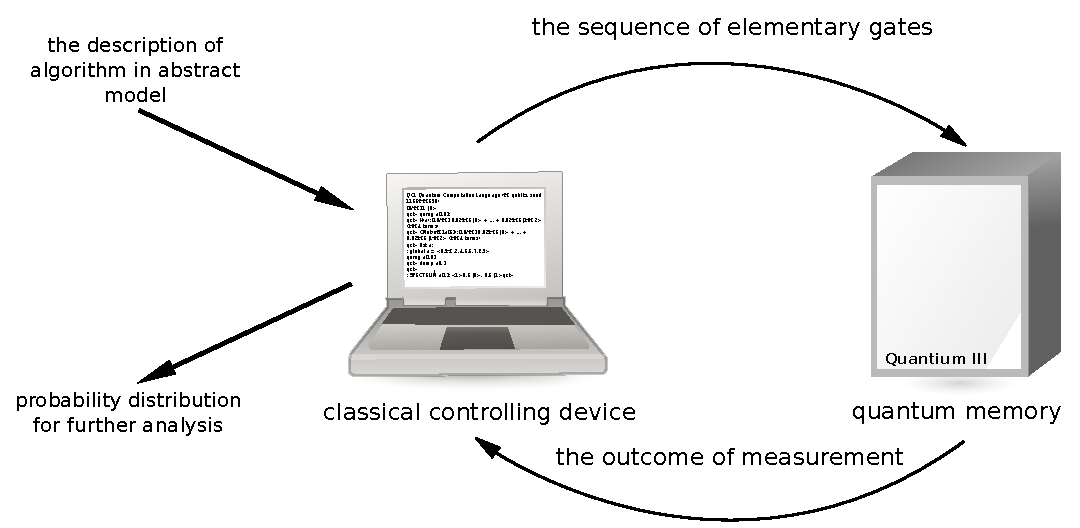
\includegraphics[width=\textwidth]{pics/qram}
\end{center}
\end{frame}

%%%%%%%%%%%%%%%%%%%%%%%%%%%%%%%%%%%%%%%%%%%%%%%%%%%%%%%%%%%%%%%%%%%%%%%%%%%%%%
\subsection{Advantages of QRAM}
%%%%%%%%%%%%%%%%%%%%%%%%%%%%%%%%%%%%%%%%%%%%%%%%%%%%%%%%%%%%%%%%%%%%%%%%%%%%%%
\begin{frame}{\insertsection}{\insertsubsection}
\begin{itemize}
	\item<1-> data abstraction \only<2->{$\equiv$ allocation of quantum memory}
	\item<3-> compound quantum operations \only<1-3>{\phantom{$\equiv$ 
	functions encapsulating sequence of quantum gates or quantum primitives}}%
    \only<4->{$\equiv$ functions encapsulating sequence of quantum gates or 
    quantum primitives}
	\item<5-> classical control of quantum operations
    \only<1-5>{\phantom{$\equiv$ loops, ifs etc. mixed with quantum code}}%
    \only<6->{$\equiv$ loops, ifs etc. mixed with quantum code}
\end{itemize}

\end{frame}

%%%%%%%%%%%%%%%%%%%%%%%%%%%%%%%%%%%%%%%%%%%%%%%%%%%%%%%%%%%%%%%%%%%%%%%%%%%%%%
\subsection{Software architecture}
%%%%%%%%%%%%%%%%%%%%%%%%%%%%%%%%%%%%%%%%%%%%%%%%%%%%%%%%%%%%%%%%%%%%%%%%%%%%%%
%%%%%%%%%%%%%%%%%%%%%%%%%%%%%%%%%%%%%%%%%%%%%%%%%%%%%%%%%%%%%%%%%%%%%%%%%%%%%%
\begin{frame}{\insertsection}{\insertsubsection}
    
\begin{center}
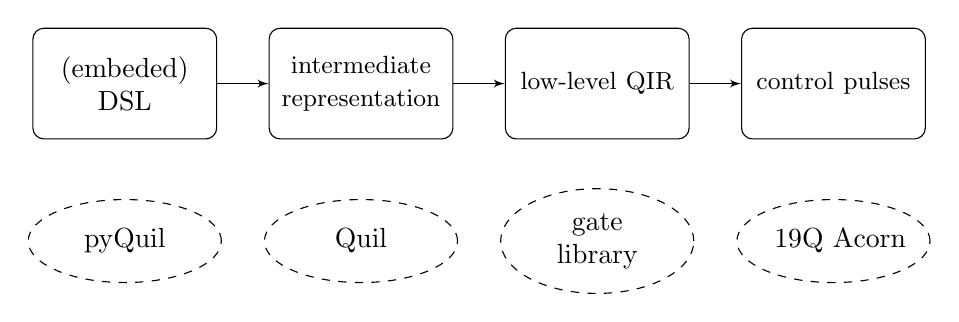
\begin{tikzpicture}[node distance = 3cm, auto]
\tikzstyle{block} = [rectangle, draw, text width=2.1cm, text centered, rounded 
corners, minimum height=4em]
\tikzstyle{example} = [draw, ellipse, node distance=2cm,  text width=1.5cm, 
dashed,
text centered, minimum  height=3em]
\tikzstyle{line} = [draw, -latex', thin]

\node [block] (edsl) {(embeded) DSL};
\node [example, below of=edsl] (edsl-ex) {pyQuil};

\node [block, right of=edsl] (qir) {\small intermediate representation};
\node [example, below of=qir] (qir-ex) {Quil};

\node [block, right of=qir] (qoptim) {\small low-level QIR};
\node [example, below of=qoptim] (qoptim-ex) {gate library};

\node [block, right of=qoptim] (qcontrol) {\small control pulses};
\node [example, below of=qcontrol] (qcontrol-ex) {19Q~Acorn};

\path [line] (edsl) -- (qir);
\path [line] (qir) -- (qoptim);
\path [line] (qoptim) -- (qcontrol);
\end{tikzpicture}
\end{center}
\end{frame}

%%%%%%%%%%%%%%%%%%%%%%%%%%%%%%%%%%%%%%%%%%%%%%%%%%%%%%%%%%%%%%%%%%%%%%%%%%%%%%
\section{Direct programming of QRAM}
%%%%%%%%%%%%%%%%%%%%%%%%%%%%%%%%%%%%%%%%%%%%%%%%%%%%%%%%%%%%%%%%%%%%%%%%%%%%%%

%%%%%%%%%%%%%%%%%%%%%%%%%%%%%%%%%%%%%%%%%%%%%%%%%%%%%%%%%%%%%%%%%%%%%%%%%%%%%%
\subsection{Quantum middelware}
%%%%%%%%%%%%%%%%%%%%%%%%%%%%%%%%%%%%%%%%%%%%%%%%%%%%%%%%%%%%%%%%%%%%%%%%%%%%%%
\begin{frame}{\insertsection}{\insertsubsection}
	\begin{itemize}
		\item embedded domain specific language $\rightarrow$ 
		C/Python/Wolfram 
		with library of functions
		\item data abstraction $\rightarrow$ allocation of classical and quantum registers based on qu(b$|$d)its
		\item quantum functions $\rightarrow$ custom elementary gates defined by matrices or compound statements
		\item classical control of quantum memory $\rightarrow$ by using host language
	\end{itemize}
\end{frame}

%%%%%%%%%%%%%%%%%%%%%%%%%%%%%%%%%%%%%%%%%%%%%%%%%%%%%%%%%%%%%%%%%%%%%%%%%%%%%%
\subsection{...its advantages...}
%%%%%%%%%%%%%%%%%%%%%%%%%%%%%%%%%%%%%%%%%%%%%%%%%%%%%%%%%%%%%%%%%%%%%%%%%%%%%%
\begin{frame}{\insertsection}{\insertsubsection}
	\begin{itemize}
        \item<1-> easy to learn and use
		\item<2-> auto-magic quantum memory management
	\end{itemize}
\end{frame}

%%%%%%%%%%%%%%%%%%%%%%%%%%%%%%%%%%%%%%%%%%%%%%%%%%%%%%%%%%%%%%%%%%%%%%%%%%%%%%
\subsection{...and its disadvantages}
%%%%%%%%%%%%%%%%%%%%%%%%%%%%%%%%%%%%%%%%%%%%%%%%%%%%%%%%%%%%%%%%%%%%%%%%%%%%%%
\begin{frame}{\insertsection}{\insertsubsection}
    \begin{itemize}
        \item very similar to low-level code
        \item lack of expressibility
    \end{itemize}
\end{frame}

%%%%%%%%%%%%%%%%%%%%%%%%%%%%%%%%%%%%%%%%%%%%%%%%%%%%%%%%%%%%%%%%%%%%%%%%%%%%%%
\subsection{Example 1: ProjectQ}
%%%%%%%%%%%%%%%%%%%%%%%%%%%%%%%%%%%%%%%%%%%%%%%%%%%%%%%%%%%%%%%%%%%%%%%%%%%%%%

\begin{frame}{\insertsection}{\insertsubsection}
	\begin{itemize}
        \item Python library developed by ETH (\url{https://projectq.ch/})
        \item offers various targets
        \begin{itemize}
            \item hardware (IBM Q Experience)
            \item resource counter (???)
            \item graphical circuit representation
        \end{itemize}
    \end{itemize}
\end{frame}

%%%%%%%%%%%%%%%%%%%%%%%%%%%%%%%%%%%%%%%%%%%%%%%%%%%%%%%%%%%%%%%%%%%%%%%%%%%%%%
\begin{frame}{\insertsection}{\insertsubsection}
	
\end{frame}

%%%%%%%%%%%%%%%%%%%%%%%%%%%%%%%%%%%%%%%%%%%%%%%%%%%%%%%%%%%%%%%%%%%%%%%%%%%%%%
\begin{frame}{\insertsection}{\insertsubsection}
	
\end{frame}

%%%%%%%%%%%%%%%%%%%%%%%%%%%%%%%%%%%%%%%%%%%%%%%%%%%%%%%%%%%%%%%%%%%%%%%%%%%%%%
\begin{frame}{\insertsection}{\insertsubsection}
	
\end{frame}


%%%%%%%%%%%%%%%%%%%%%%%%%%%%%%%%%%%%%%%%%%%%%%%%%%%%%%%%%%%%%%%%%%%%%%%%%%%%%%
\subsection{Example 2: Rigetti Forest and pyQuil}
%%%%%%%%%%%%%%%%%%%%%%%%%%%%%%%%%%%%%%%%%%%%%%%%%%%%%%%%%%%%%%%%%%%%%%%%%%%%%%

\begin{frame}{\insertsection}{\insertsubsection}
	
\end{frame}

%%%%%%%%%%%%%%%%%%%%%%%%%%%%%%%%%%%%%%%%%%%%%%%%%%%%%%%%%%%%%%%%%%%%%%%%%%%%%%
\begin{frame}{\insertsection}{\insertsubsection}
	
\end{frame}

%%%%%%%%%%%%%%%%%%%%%%%%%%%%%%%%%%%%%%%%%%%%%%%%%%%%%%%%%%%%%%%%%%%%%%%%%%%%%%
\begin{frame}{\insertsection}{\insertsubsection}
	
\end{frame}

%%%%%%%%%%%%%%%%%%%%%%%%%%%%%%%%%%%%%%%%%%%%%%%%%%%%%%%%%%%%%%%%%%%%%%%%%%%%%%
\begin{frame}{\insertsection}{\insertsubsection}
	
\end{frame}

%%%%%%%%%%%%%%%%%%%%%%%%%%%%%%%%%%%%%%%%%%%%%%%%%%%%%%%%%%%%%%%%%%%%%%%%%%%%%%
\section{High-level programming}
%%%%%%%%%%%%%%%%%%%%%%%%%%%%%%%%%%%%%%%%%%%%%%%%%%%%%%%%%%%%%%%%%%%%%%%%%%%%%%


%%%%%%%%%%%%%%%%%%%%%%%%%%%%%%%%%%%%%%%%%%%%%%%%%%%%%%%%%%%%%%%%%%%%%%%%%%%%%%
\subsection{Domain specific languages}
%%%%%%%%%%%%%%%%%%%%%%%%%%%%%%%%%%%%%%%%%%%%%%%%%%%%%%%%%%%%%%%%%%%%%%%%%%%%%%

\begin{frame}{\insertsection}{\insertsubsection}
    
\begin{block}{Level 2}
Domain specific language with data and function abstraction
\end{block}

\begin{itemize}
    \item QCL (\url{http://tph.tuwien.ac.at/~oemer/qcl.html})
    \item LanQ (\url{http://lanq.sourceforge.net/})
    \item QPL anc cQPL (\url{https://arxiv.org/abs/quant-ph/0511145})
\end{itemize}
\end{frame}


%%%%%%%%%%%%%%%%%%%%%%%%%%%%%%%%%%%%%%%%%%%%%%%%%%%%%%%%%%%%%%%%%%%%%%%%%%%%%%
\subsection{Example 1: QCL -- focus on quantum computing}
%%%%%%%%%%%%%%%%%%%%%%%%%%%%%%%%%%%%%%%%%%%%%%%%%%%%%%%%%%%%%%%%%%%%%%%%%%%%%%

\begin{frame}{\insertsection}{\insertsubsection}
	\begin{itemize}
		\item first release in 1998, last in 2014 
		(\url{http://tph.tuwien.ac.at/~oemer/qcl.html})
		\item architecture independent programming language for quantum computers
		\item quantum operators and quantum functions
		\item quantum conditions
	\end{itemize}
	
\end{frame}

%%%%%%%%%%%%%%%%%%%%%%%%%%%%%%%%%%%%%%%%%%%%%%%%%%%%%%%%%%%%%%%%%%%%%%%%%%%%%%
\begin{frame}{\insertsection}{\insertsubsection}
	
\end{frame}

%%%%%%%%%%%%%%%%%%%%%%%%%%%%%%%%%%%%%%%%%%%%%%%%%%%%%%%%%%%%%%%%%%%%%%%%%%%%%%
\begin{frame}{\insertsection}{\insertsubsection}
	
\end{frame}

%%%%%%%%%%%%%%%%%%%%%%%%%%%%%%%%%%%%%%%%%%%%%%%%%%%%%%%%%%%%%%%%%%%%%%%%%%%%%%
\begin{frame}{\insertsection}{\insertsubsection}
	
\end{frame}


%%%%%%%%%%%%%%%%%%%%%%%%%%%%%%%%%%%%%%%%%%%%%%%%%%%%%%%%%%%%%%%%%%%%%%%%%%%%%%
\subsection{Example 2: cQPL -- focus on quantum communication}
%%%%%%%%%%%%%%%%%%%%%%%%%%%%%%%%%%%%%%%%%%%%%%%%%%%%%%%%%%%%%%%%%%%%%%%%%%%%%%

%%%%%%%%%%%%%%%%%%%%%%%%%%%%%%%%%%%%%%%%%%%%%%%%%%%%%%%%%%%%%%%%%%%%%%%%%%%%%%
\begin{frame}{\insertsection}{\insertsubsection}
    
\end{frame}

%%%%%%%%%%%%%%%%%%%%%%%%%%%%%%%%%%%%%%%%%%%%%%%%%%%%%%%%%%%%%%%%%%%%%%%%%%%%%%
\begin{frame}{\insertsection}{\insertsubsection}
    
\end{frame}

%%%%%%%%%%%%%%%%%%%%%%%%%%%%%%%%%%%%%%%%%%%%%%%%%%%%%%%%%%%%%%%%%%%%%%%%%%%%%%
\begin{frame}{\insertsection}{\insertsubsection}
    
\end{frame}

%%%%%%%%%%%%%%%%%%%%%%%%%%%%%%%%%%%%%%%%%%%%%%%%%%%%%%%%%%%%%%%%%%%%%%%%%%%%%%
\section{Where are quantum computers?}
%%%%%%%%%%%%%%%%%%%%%%%%%%%%%%%%%%%%%%%%%%%%%%%%%%%%%%%%%%%%%%%%%%%%%%%%%%%%%%

%%%%%%%%%%%%%%%%%%%%%%%%%%%%%%%%%%%%%%%%%%%%%%%%%%%%%%%%%%%%%%%%%%%%%%%%%%%%%%
\begin{frame}{\insertsection}
	\begin{itemize}
		\item D-Wave (GOTO: Andy Mason and Sheir Yarkoni, Tutorial on 
		programming the D-Wave system) 
		\item IBM (GOTO: Ram Du\v{s}i\'c Hren, IBM Q Experience: Hands-on 
		workshop)
		\item Rigetti (Quil language embedded in Python)
		\item ProjectQ -- various back-ends: simulator, resource counter, 
		hardware (at the moment targeting IBM Q Experience)
	\end{itemize}
\end{frame}


%%%%%%%%%%%%%%%%%%%%%%%%%%%%%%%%%%%%%%%%%%%%%%%%%%%%%%%%%%%%%%%%%%%%%%%%%%%%%%
\section{Q?}
%%%%%%%%%%%%%%%%%%%%%%%%%%%%%%%%%%%%%%%%%%%%%%%%%%%%%%%%%%%%%%%%%%%%%%%%%%%%%%
%%%%%%%%%%%%%%%%%%%%%%%%%%%%%%%%%%%%%%%%%%%%%%%%%%%%%%%%%%%%%%%%%%%%%%%%%%%%%%
\begin{frame}{\insertsection}
    \begin{center}
        \Huge {\color{iitis-orange} \insertsection}\\[12pt]
        \LARGE Thank you.
    \end{center}
\end{frame}

\end{document}
